\section{Methodology}
\label{sec:method}
%\FloatBarrier

The system consists of two separate parts; an unsupervised algorithm for
augmenting data, and a supervised algorithm for classifying the data
(Figure~\ref{fig:overview}). The unsupervised portion attempts to augment the
data with additional structural information. It could be considered a
preprocessing step, with the choice of parameters acting as a way to inject some
amount of domain knowledge into the data. The supervised portion consists of a
regular classification algorithm. \todo[inline]{Todo: Rewrite this and add all
  the details about how the data is used (sliding window, stratified sampling, etc)}

\begin{figure}[htb]
  \centering
  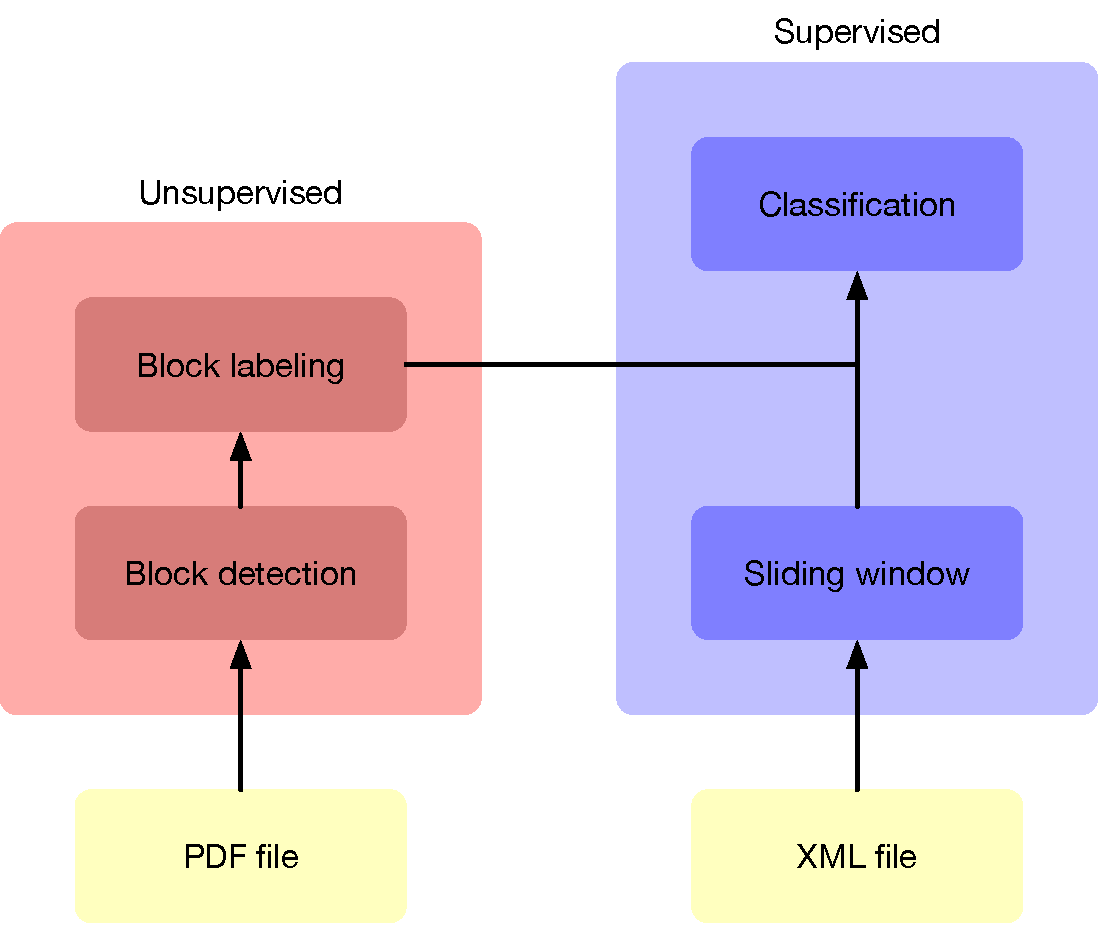
\includegraphics[width=\textwidth]{figures/layout.pdf}
  \caption{A high-level overview of the system}
  \label{fig:overview}
\end{figure}

\subsection{Unsupervised}
The unsupervised algorithm attempts to detect and label blocks of text in the
PDF file, as shown in Figure~\ref{fig:clustered} for an example). This approach
is based on work by \textcite{klampfl2014unsupervised}, and consists of two
clustering steps:
\begin{enumerate}
\item Individual letters are clustered together into blocks of semantically
  relevant text (e.g. a full paragraph, or a section header).
\item These blocks are labeled by a different clustering algorithm.
\end{enumerate}

\begin{figure}[htb]
  \centering
  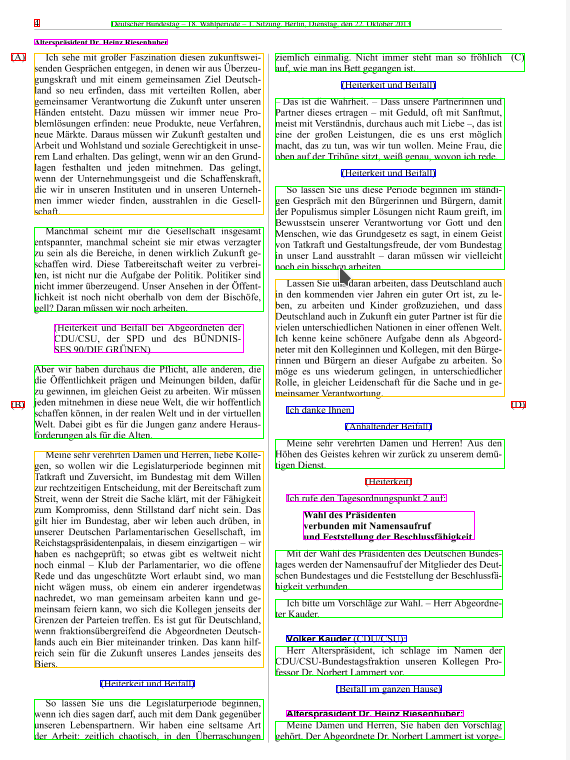
\includegraphics[height=0.5\textheight]{figures/cluster_example.png}
  \caption{An example of clustered blocks of text, blocks with the same outline
    color belonging to the same cluster.}
  \label{fig:clustered}
\end{figure}

\subsubsection{Hierarchical Agglomerative Clustering}
The first step is performed using hierarchical agglomerative clustering (HAC),
an unsupervised bottom-up clustering algorithm that constructs a hierarchical
tree of clusters (in this context referred to as a \emph{dendrogram}). An
example is shown in Figure~\ref{fig:hac}. The algorithm gets fed the individual
characters present in the PDF files, then iteratively groups the two closest
clusters (the initial inputs being regarded as clusters of one element) together
until only a single cluster remains. This process involves two parameters:
\begin{enumerate}
\item The distance function between two characters.
\item The distance function between two groups of characters.
\end{enumerate}
The first parameter is trivially chosen to be the Euclidian distance between the
coordinates of the two characters. The second parameter is called the
\emph{linkage} and has several common options, the most basic of which are:
\begin{itemize}
\item Single-linkage: The distance between groups is based on the closest two
  elements: \[ d(A, B) = \min \{ d(a, b) : a \in A, b \in B \} \]
\item Maximum-linkage: The distance between groups is based on the furthest two
  elements: \[ d(A, B) = \max \{ d(a, b) : a \in A, b \in B \} \]
\item Average-linkage: The distance between groups is based on the average
  distance of its elements:
  \[ d(A, B) = \frac{1}{|A||B|} \sum_{a \in A}\sum_{b \in B} d(a, b) \]
\end{itemize}
As per \textcite{klampfl2014unsupervised}, single-linkage clustering performs
best for this task due to its tendency to form long thin clusters, mimicking the
structure of sentences. As an additional bonus, while the general time
complexity for HAC is in $\mathcal{O}(n^3)$, single-linkage clustering can be
done in $\mathcal{O}(n^2)$ \citep{sibson1973slink}, making it far more usable on
realistic datasets.

\begin{figure}[htb]
  \centering
  \begin{subfigure}[b]{0.40\textwidth} 
    \centering
    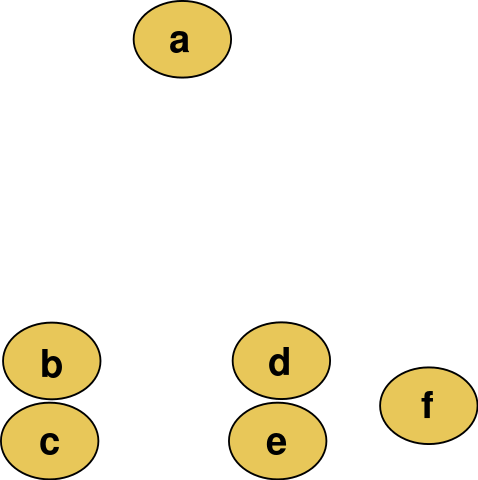
\includegraphics[width=\textwidth]{figures/dendrogram1.png}
    \caption{Before}
  \end{subfigure}
  \hspace{0.10\textwidth}
  \begin{subfigure}[b]{0.40\textwidth}
	\centering
    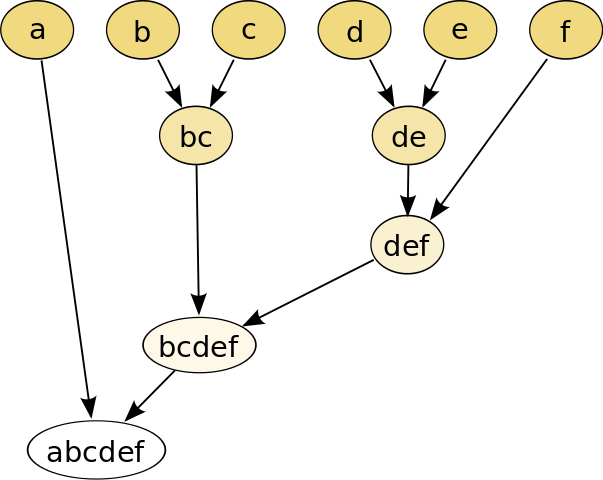
\includegraphics[width=\textwidth]{figures/dendrogram2.png}
    \caption{After}
  \end{subfigure}
  \caption{An example of hierarical agglomerative clustering.}
  \label{fig:hac}
\end{figure}

After the dendrogram is constructed, the only choice left is at which level to
cut the tree to obtain the desired blocks of text. This is left as a parameter
to be manually fine-tuned.

\subsubsection{Classical Clustering}
The extracted blocks from the previous step are then clustered according to
the similarity of their shapes (width and height). This is done using K-means
clustering for some chosen $K$, or with the DBSCAN algorithm.
\todo[inline]{Todo: Either expand this section or just integrate it with the previous subsection.}

\subsection{Supervised}
\todo[inline]{This is written as a draft}
\todo[inline]{Cite a survey mentioning these methods}

After the data is augmented by the previously described clustering algorithm,
it's fed into a supervised classifier. For the purposes of machine learning,
text produces 3-dimensional data: there is a feature vector for each word, and
some (either variable or predetermined through padding) amount of words per
text. This makes each training sample a 2-dimensional matrix, which then gets
stacked in the depth dimension to produce 3-dimensional training data. This is
troublesome as the standard machine learning algorithms work on 2-dimensional
data, assuming a feature vector for each sample rather than a matrix. There are
three common methods to deal with this:
\begin{itemize}
\item Bag of words
\item Convolutional neural networks
\item Recurrent neural networks
\end{itemize}

Aside from being completely different methods, they differ in a major way in how
they handle the sequential nature of text. The bag of words approach is the
simplest in that it simply disregards this sequential nature, instead creating
what is essentially a histogram of word occurrences. This downsamples each
sample from a feature matrix to a feature vector, allowing the use of normal
machine learning algorithms (commonly support vector machines). While the
sequential information can be kept to some degree by use histograms of $n$-grams
rather than words (unigrams), this causes the size of the input data to scale
exponentially with the value of $n$.

Convolutional neural networks (CNNs) work by taking a number of filters
(sometimes called kernels or feature maps) of a specified size and convolving
these over the input data. A simplified example using one filter is shown in
Figure~\ref{fig:cnn}.
\begin{figure}[htb]
  \centering
  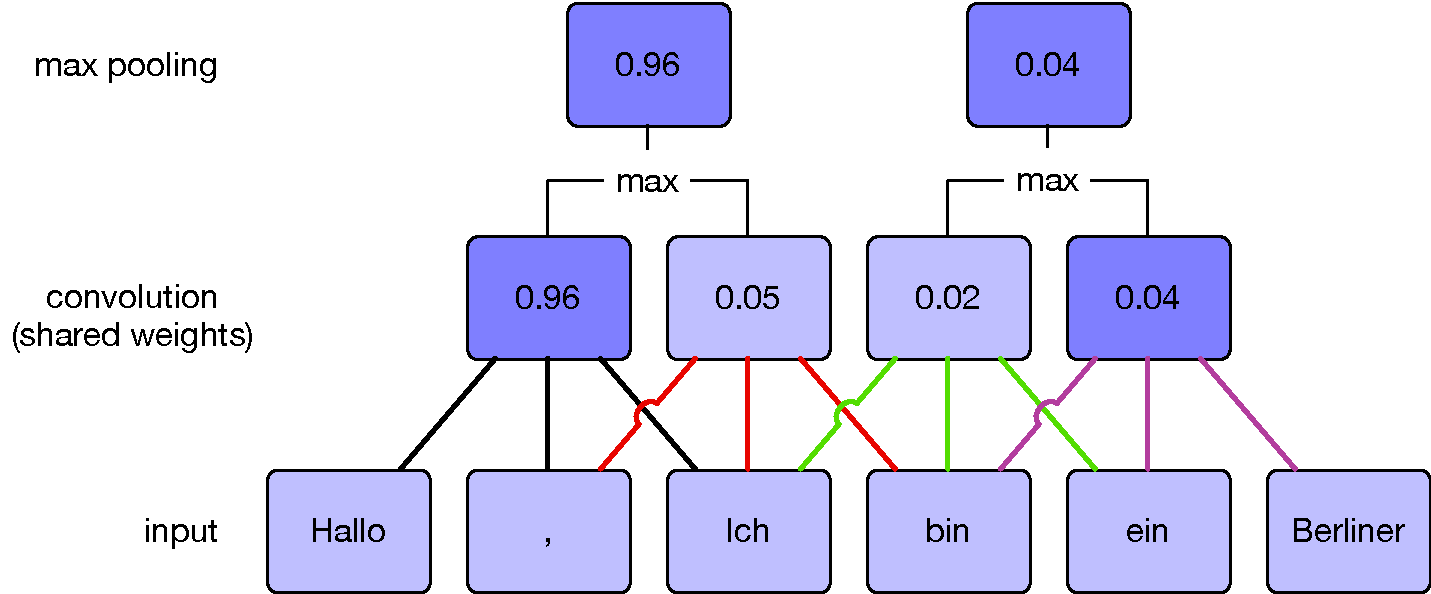
\includegraphics[width=\textwidth]{figures/cnn.pdf}
  \caption{A simplified convolutional neural network}
  \label{fig:cnn}
\end{figure}
In this example, the input text is convolved with a filter with a width of 3 and
a stride of 1 --- that is, each application of the filter considers three
subsequent input elements, after which the window is shifted one space to the
right. This filter is essentially a small neural network mapping three items to
one output value, whose weights are reused for each application of the filter.
Reusing the weights in this way (weight sharing) prevents the number of
parameters in the network from spiraling out of control.
\citep{lecun1995convolutional} After the application of this convolution layer,
the responses of the filter form a new sequence of roughly the same size as the
input (minus a few due to missing the edges). The next step is to downsample
this sequence by means of a \emph{max pooling} layer, which maps all values
within a window to the maximum value amongst those values. While conceptually
similar to a convolution, this step generally does not involve overlap, instead
either setting the stride to the same value as the window size (usually 2)
reducing the entire sequence to 1 value (1-max pooling). The reason for this is
twofold:
\begin{enumerate}
\item It downsamples the number of inputs, reducing the amount of parameters
  required further on in the network.
\item It adds translation invariance to the feature detected by this filter. The
  example filter of Figure~\ref{fig:cnn} appears to react strongly to the
  presence of the word ``Hallo''. Without the pooling layer, changing the
  location of the word ``Hallo'' in the input would similarly change the
  location of the high activation in the intermediate representation; this would
  be \emph{equivariance}. The more aggressively the pooling is applied, the
  higher the degree of invariance.
\end{enumerate}
This combination of convolution followed by pooling can be repeated multiple
times as desired or until there is only a single value left as output from the
filter. Finally, the outputs of all filters are concatenated and fed into a
standard feedforward neural network.

While CNN architectures in computer vision are generally very deep, they tend to
be very shallow in natural language processing; commonly just a single
convolution followed by 1-max pooling \citep{zhang2015conv}. Since this
particular task at first glance appears to be fairly reliant on word position
(e.g. a colon at the end of a sentence very often indicates the start of a
speech, a colon in the middle almost certainly does not), the degree of pooling
will be experimented with.

\subsubsection{Difference between convolutional and recurrent neural networks}
Recurrent neural networks (in particular LSTMs or GRUs) are seemingly the most
natural fit for language processing, since they process an entire sequence and
are therefore fully conditioned on the word order (as opposed to the
convolutional neural networks which tend to learn translation invariant ngram
features). Regardless, convolutional neural networks will be used in this
research. This choice is based on two factors:
\begin{enumerate}
\item In practise, the performance for classification tasks does not differ
  between the two types of networks.\citep{cnnrnn}
\item The computations in convolutional networks are highly independent of
  each other, allowing for great paralellization (in particular with regards to
  running on a GPU). In contrast, LSTMs are bottlenecked by the fact that each
  calculation is dependent on the previous calculations. As a result, CNNs
  achieve far higher training speeds.\citep{facebook}
\end{enumerate}

\todo[inline]{Diagram/description of the full model with cluster labels added}

%%% Local Variables:
%%% mode: latex
%%% TeX-master: "report"
%%% End:
